% ------------------------------------------------------------------------
% 40. Theory
% ------------------------------------------------------------------------

\chapter{Theory}
\label{chap:theory}

In this chapter, key background concepts and methodologies used in the thesis are going to be discussed. The chapter is going to explain what is meant by unmanned aerial system and its components.

The chapter is also going to discuss on the cloud provider, Amazon web services (AWS), used to host various components of developed system, simulation and software development tools used, as well as laws and regulations around unmanned aerial systems.

\section{Unmanned Aerial System}
\label{sec:unmanned-aerial-system}

An unmanned aerial system commonly referred to as UAS is a set of an unmanned aerial vehicle and compononents that support its operations. They do not carry human pilots but are piloted remotely or autonomously. A UAS is usually comprised of four main components namely,

\begin{itemize}
    \item An unmanned aerial vehicle also known as a UAV.
    \item A ground control station also known as a GCS, from where human pilots can remotely pilot a UAV or upload mission payload for the UAV to execute autonomously.
    \item Sensors and devices specific to the aerial vehicles' intended mission. These can be cameras or other various sensors.
    \item A datalink between a UAV and a GCS.
\end{itemize}

A typical UAS also includes some ways to collect telemetry from the UAV to some sort of datalake for further analysis. The collected data can be used for machine learning to improve the UAV operational efficiency.

<ADD AN IMAGE THAT SHOWS A TYPICAL UAS>

\subsection{Unmanned Aerial Vehicle}
Unmanned aerial vehicle is a term used to refer to an aerial vehicle that has no human onboard pilot but is rather piloted remotely by humans from a remote ground control station or is autonomously piloted using onboard flight algorithms. Unmanned aerial vehicles are commonly known as UAVs, drones or remotely piloted vehicles (RPV).
<ADD MORE EXPLANATION>

\subsubsection{Classification of Unmanned Aerial Vehicles}
UAVs come in different classifications depending on the frame structure, size, operational range and/or payload capacity.

Table <REFERENCE TABLE> shows how the United States Department of Defense classifies UAVs.


\section{Amazon Web Services}
Amazon Web Services, commonly known as AWS, is a cloud platform provided by Amazon that provides various service offerings such as platform as a service, PaaS, and infrastructure as a service, IaaS\cite{awswhatisaws2022}. AWS makes it easy for developers, engineers and businesses to deploy scalable, resilient, agile and highly available infrastructures for databases, servers, applications, storage, analytics, \textit{et cetera}. AWS offers attractive and cost saving payment strategies of which there are pay-as-you-go, save when you commit, and pay less by using more\cite{awspricing2022}.

AWS has a concept of regions, which refers to a phyisical location around the world, where multiple datacenters are deployed in a cluster. Each cluster of datacenter is called an availability zone\cite{awsregionsandazs}. AWS set this up like this to guarantee high availability and reliability of deployed resources.

\begin{figure}[H]
    \centering 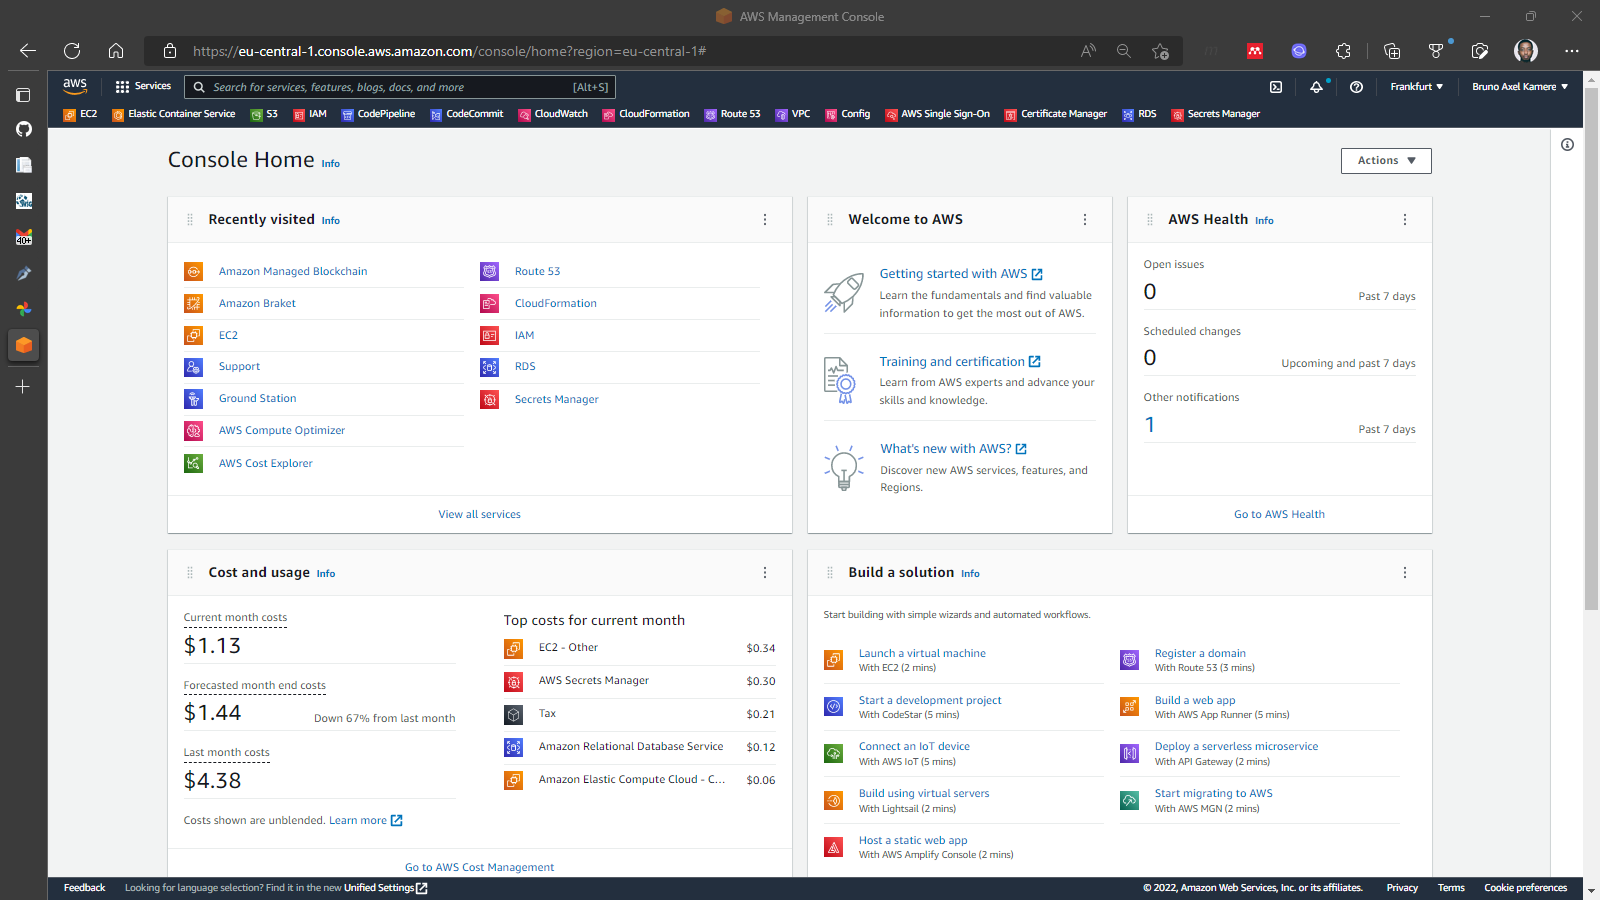
\includegraphics[width=0.9\linewidth]{aws_console_home.png}
    \caption{AWS console home.}
    \label{fig:aws-console-home}
    \source{Own work.}
\end{figure}

Cloud computing is an emerging technology that has revolutionized how businesses go online. Cloud computing has been and still is of great use in various industries, including the aerospace and energy industries. Burak et al developed a cloud and edge solution running on AWS that aimed at increasing turbine maintenance inspections' efficiency through automation and a serverless AWS architecture while reducing operations cost\cite{burakawswindfarm2021}. The solution proposed by Burak et al was comprised of drones, machine learning and internet of things processes running on cloud and edge.

The proposed solution in this thesis also takes advantage of what AWS and cloud computing offers. Several components, like the ground control system, of the proposed solution are running on AWS. See the high-high-level design in figure \ref{fig:uas-hhld}.

\subsection{Infrastructure as code}
Infrastructure as Code also known as IaC, a technique very often used in the DevOps and automation community, is an infrastructure that is provisioned through code and scripts written in familiar programming languages like Python, PHP, Node.JS, C\# \textit{et cetera}. The infrastructure deployed through code can be servers, databases, firewalls, data centers \textit{et cetera}. The main advantages of defining an infrastructure as code are:

\begin{itemize}
    \item Improved efficiency and consistency.
    \item Reduced human error.
    \item Infrastructure agility. An infrastructure defined as code can be deployed as many times as needed, which reduces the effort invested by developers in case a replica of an environment is needed elsewhere.
    \item It allows developers to take advantage of programming languages features like loops, variables \textit{et cetera} to build more agile infrastructures.
    \item The infrastructure can be versioned and tightly controlled. Since the infrastructure is basically standard code, it can be versioned with various versioning tools like Git or Subversion. This facilitates maintanance and makes the infrastructure easy to be rolled back, in case of issues.
    \item It helps with cost savings. Since the whole infrastructure is basically deployed automatically through code, engineers can then shift their focus to work on other important tasks.
\end{itemize}

In this thesis, Infrastructure as Code is used to its outmost potential. The AWS infrastructure is deployed as code using the AWS proprietary software development framework called AWS Cloud Development Kit or AWS CDK. AWS CDK is an open source kit provided by AWS that allows engineers to define IT infrastructures on AWS using familiar programming languages. In the source code \ref{code:route_53_records} is an example snippet from the AWS CDK app developed for the proposed solution in this thesis. The snippet represents a part that adds DNS records to the AWS Route 53 service using standard Python code.

\begin{center}
    \captionsetup{type=listing}
    \inputminted[
        frame=single,
        framesep=2mm,
        baselinestretch=1.2,
        fontsize=\footnotesize,
        breaklines,
        breakanywhere,
        linenos
    ]{python}{config/code/7c11d95d3b55be021475679db7f9f9dd/route_53_records.py}
    \captionof{listing}{helloskygroup.com AWS CDK Python Route 53 snippet.}
    \label{code:route_53_records}
\end{center}

\section{Simulation}
The initial project plan was to develop a whole UAS from scratch with an actual physical UAV and components, but this was deemed to be time consuming, and expensive to develop. Therefore, all the components that make a UAV were simulated using a simulation technique called Software in the loop or SITL. This technique allows developers to develop UAV flight logics using software and no hardware involved, eventhough that is possible as well. Chapter \ref{chap:methodology-and-setup} elaborates more on how SITL was used in this project to simulate an actual UAV with telemetry.

\section{Tools used}
\label{sec:tools-used}
The solution proposed in this thesis was built using various software development, and design tools. The choice of tools is really key to an organised and well managed project development, therefore it was important to choose the right tools for the right tasks to help get the expected outcome from them.

In the next subsections, various tools during the solution development are going to be listed and discussed.

\subsection{Microsoft Visual studio code}
\label{subsec:ms-visual-studio-code}
Visual studio code or VS code is a source code editor provided by Microsoft. It was used in this thesis as a code editor to write various codes and scripts.
<ADD SCREENSHOT>

\subsection{PyCharm by JetBrains}
\label{subsec:pycharm}
The AWS infrastructure was built as code using Python programming language. Due to its robustness and great Python support, Pycharm by JetBrains integrated development devolpment (IDE) was the go to choice.

\begin{figure}[H]
    \centering 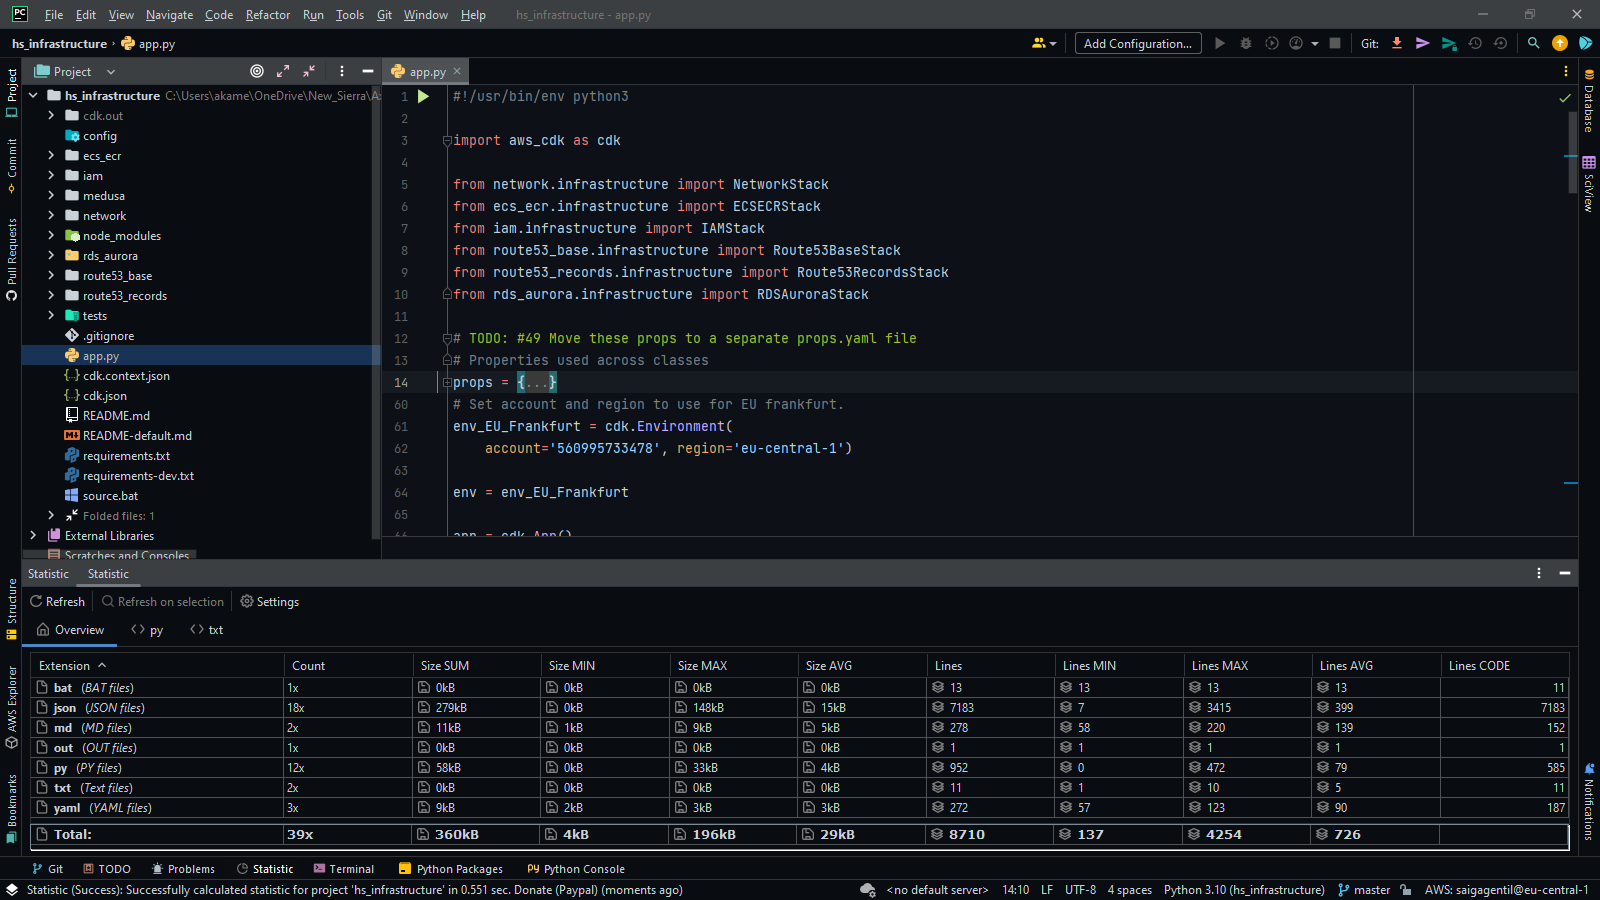
\includegraphics[width=0.9\linewidth]{pycharm_main_view.png}
    \caption{PyCharm editor.}
    \label{fig:pycharm}
    \source{Own work.}
\end{figure}

\subsection{PhpStorm by JetBrains}
\label{subsec:phpstorm}
PhpStorm is an integrated development environment created by JetBrains specifically for php programming language. The web interface from which the UAV is controlled from is built with php's Laravel framework, and PhpStorm is perfectly optimised for development of php web applications.

\begin{figure}[H]
    \centering 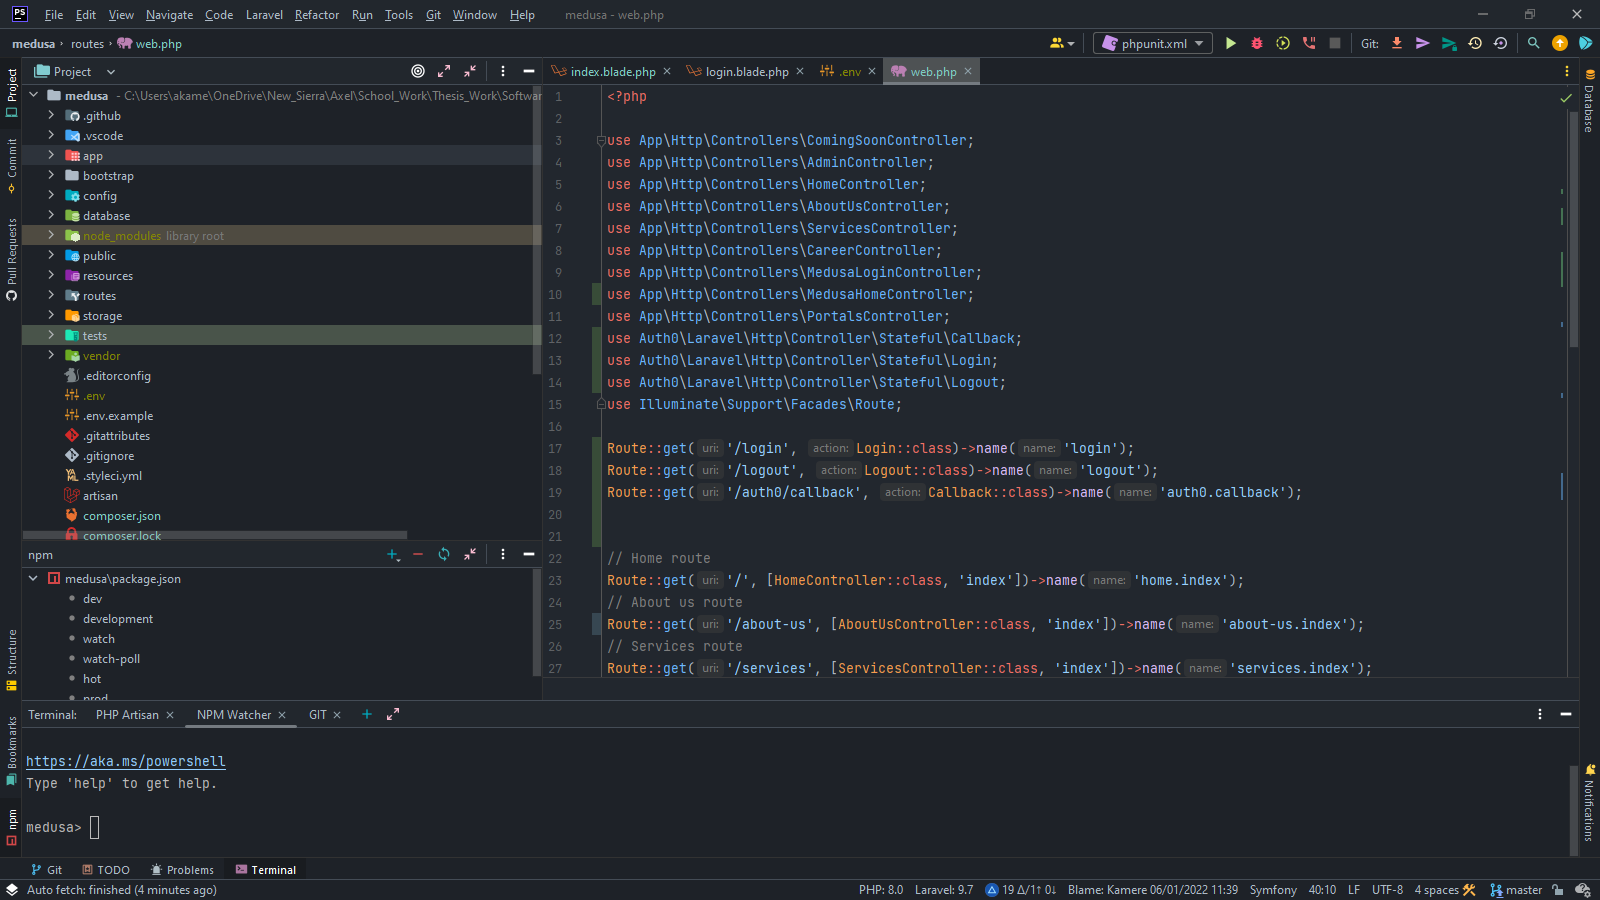
\includegraphics[width=0.9\linewidth]{phpstorm_main_view.png}
    \caption{PhpStorm editor.}
    \label{fig:phpstorm}
    \source{Own work.}
\end{figure}

\subsection{Affinity Designer}
\label{subsec:affinity-designer}
Several user interface components used across the project like icons and logos, like in figure \ref{fig:hs-group-logos} for example, were designed using Affinity Designer. Affinity Designer is a graphics tool used to design and create logos, icons, concept arts, UI designs \textit{et cetera}.

\begin{figure}[H]
    \centering 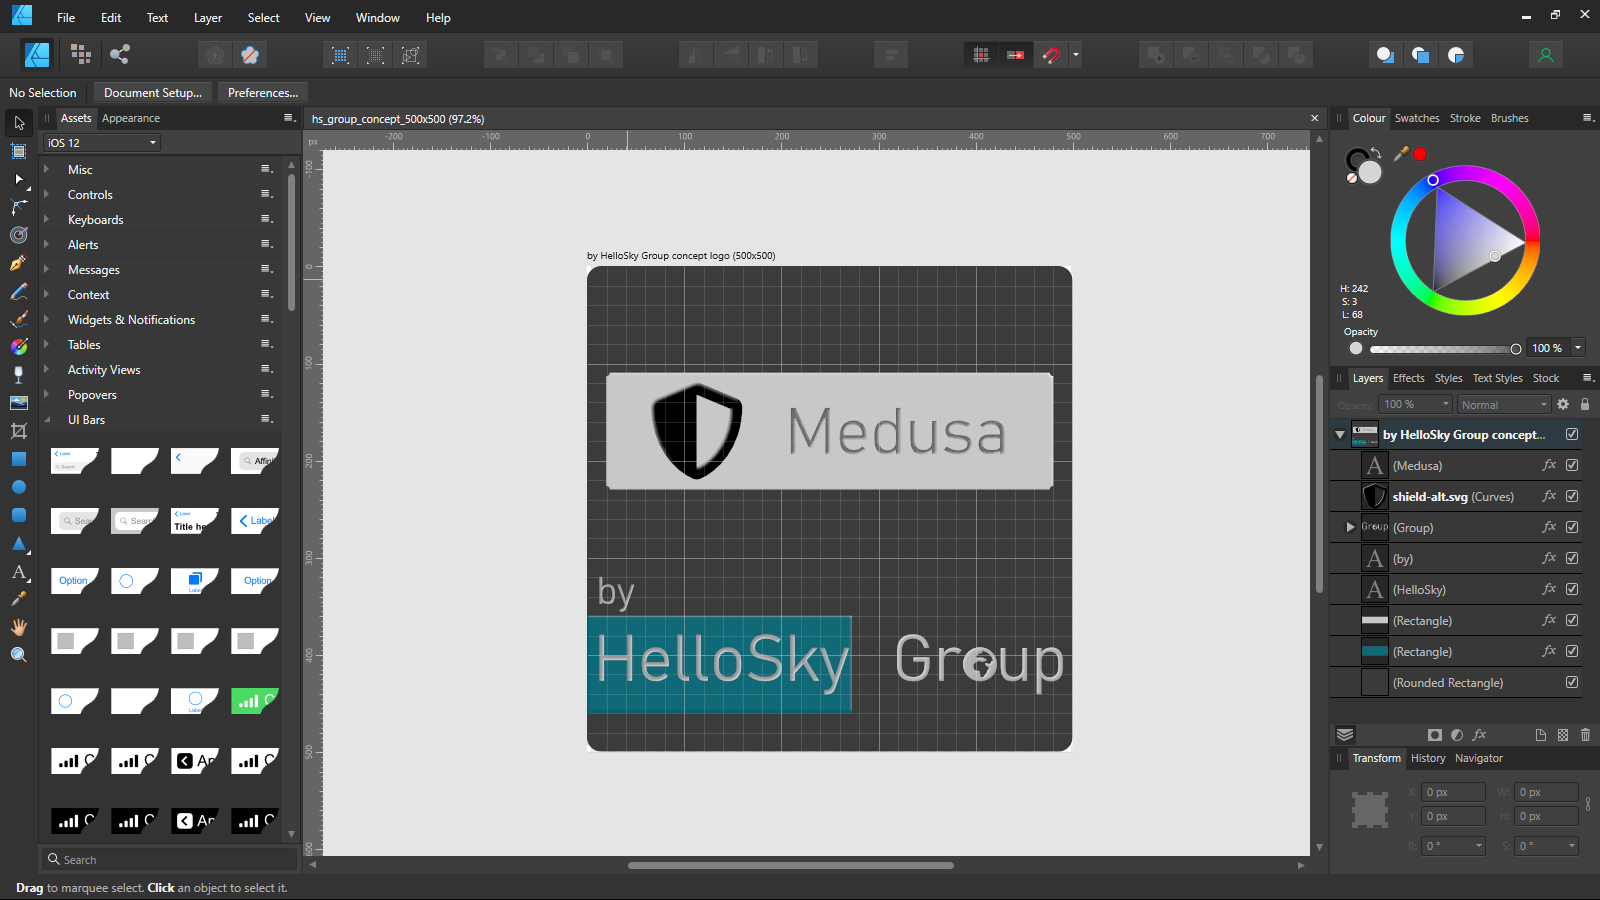
\includegraphics[width=0.9\linewidth]{affinity_designer_main_view.png}
    \caption{Affinity Designer editor.}
    \label{fig:affinity-designer}
    \source{Own work.}
\end{figure}

\subsection{GitHub}
\label{subsec:github}
One of the fundamentals of software development and coding projects generally is to version the code so that changes can be tracked overtime. Making sure that a project is versioned and maintained centrally in a repository is very important, especially where teams are working together on a similar project. Git, one of the softwares used for code versioning, was used in this project to track changes across various components of the overall project. In fact this thesis document itself is versioned using Git <ADD LINK TO THIS THESIS ON GITHUB>, alongside other components of the proposed solution. Github then comes into play to act as the single point of truth where multiple Git repositories can be pushed and managed from.
<ADD IMAGE SHOWING A TYPICAL BASIC GIT - GITHUB FLOW>

\begin{figure}[H]
    \centering 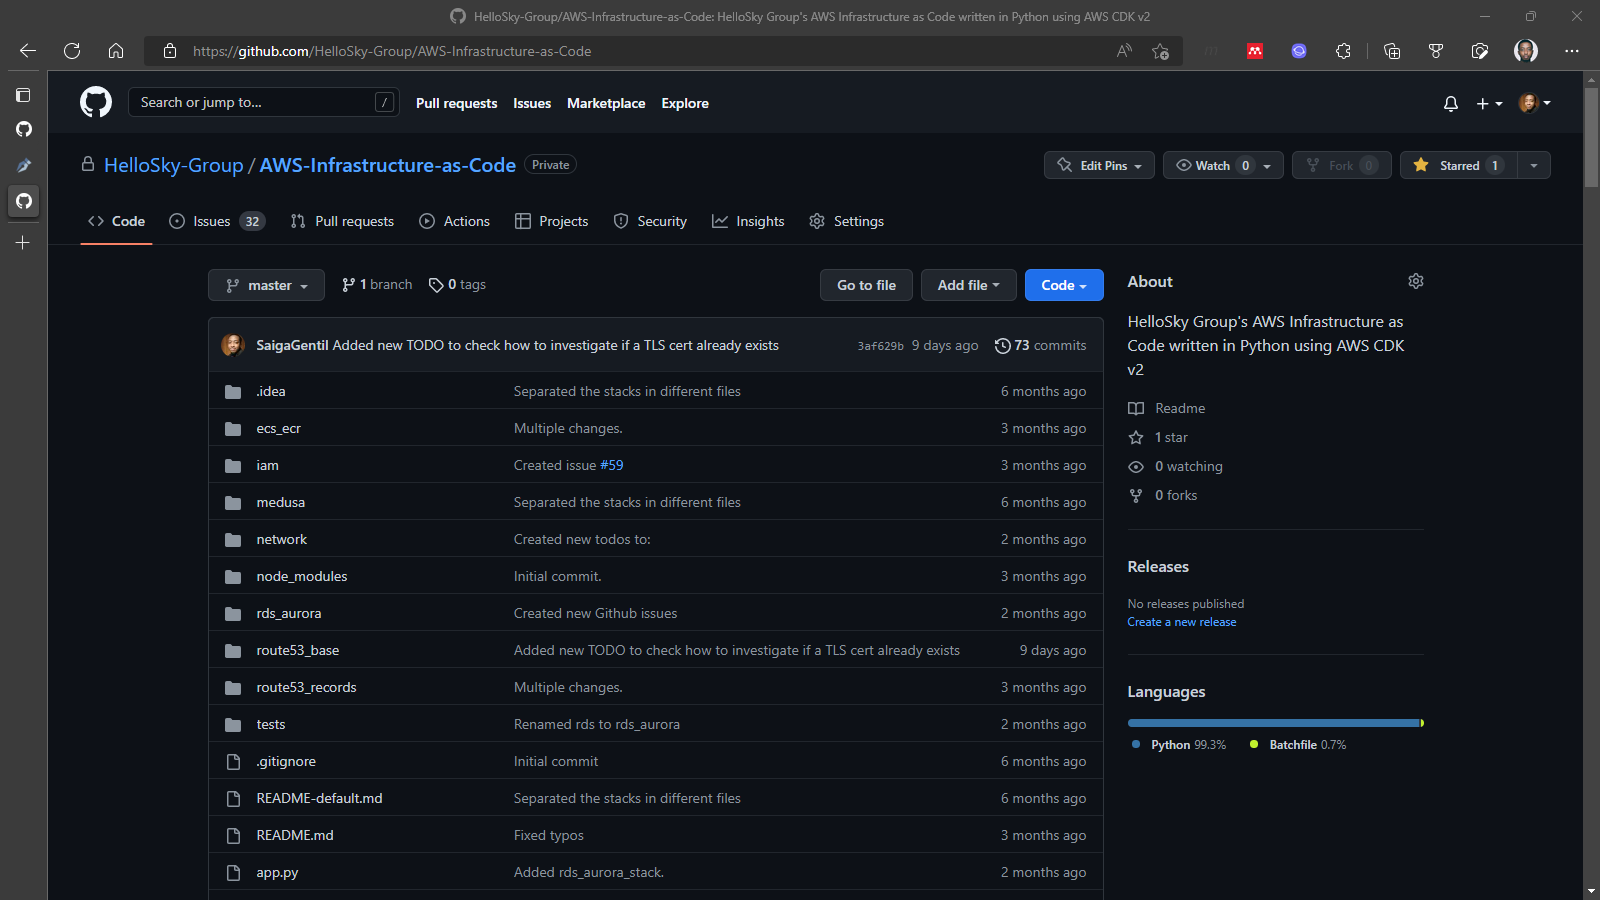
\includegraphics[width=0.9\linewidth]{github_main_view.png}
    \caption{Github repository for the AWS infrastructure code.}
    \label{fig:github}
    \source{Own work.}
\end{figure}

\subsection{Microsoft Visio}
\label{subsec:ms-visio}
Microsoft Visio is an application part of the Microsoft office family that is used for digramming and graphics visualization. It is used to build architecture diagrams and many more. In this project, Microsoft Visio was used to design and create architecture design diagrams of the proposed solution.

\begin{figure}[H]
    \centering 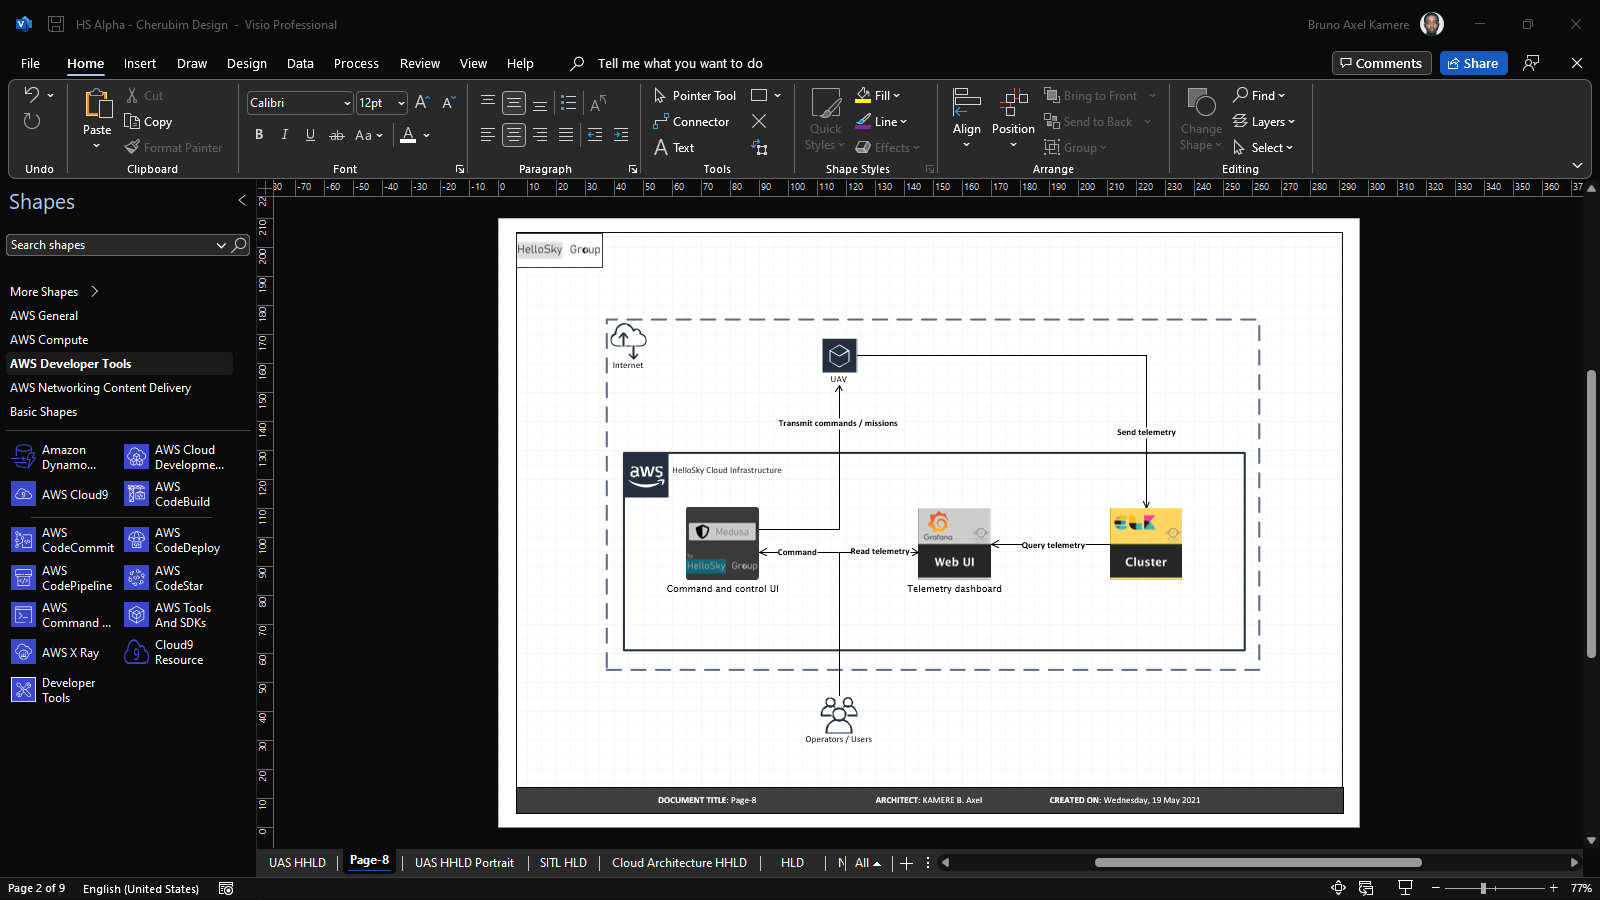
\includegraphics[width=0.9\linewidth]{ms_visio_main_view.png}
    \caption{Microsoft Visio.}
    \label{fig:ms-visio}
    \source{Own work.}
\end{figure}

% \section{Law and regulation}
% The aerospace industry is one of the highly regulated industries. And this is so for a reason, mainly safety and airspace security.
% <FINISH SECTION>.

\nomenclature[z-IaaS]{IaaS}{Infrastructure as a Service}
\nomenclature[z-PaaS]{PaaS}{Platform as a Service}
\nomenclature[z-ML]{ML}{Machine Learning}
\nomenclature[z-ML]{ML}{Machine Learning}
\nomenclature[z-IaC]{IaC}{Infrastructure as Code}
\nomenclature[z-CDK]{CDK}{Cloud Development Kit}
